% Options here are passed to the article class.
% Most common options: 10pt, 11pt, 12pt
\documentclass[10pt]{datasheet}

% Input encoding and typographical rules for English language
\usepackage[utf8]{inputenc}
\usepackage[english]{babel}
\usepackage[english]{isodate}

% tikz is used to draw images in this example, but you can
% also use \includegraphics{}.
\usepackage{graphicx}

% These define global texts that are used in headers and titles.
\title{WI02: Instant Upwards Comparator Wire}
\author{Andrews54757}
\tags{wiring, instant-comparator}
\date{21 December 2022}
\revision{Revision 1}
\begin{document}
\maketitle

\section{Features}

\begin{itemize}
\item{Constant time on/off for all signal strengths < 15}
\item{8gt throughput}
\item{Can input from multiple places}
\end{itemize}

\section{Applications}

\begin{itemize}
\item{Vertical signal transport.}
\end{itemize}

\section{General Description}
Transports signals upwards in constant time. Horizontal area of 10x3. Can input from multiple places as shown in schem.

\vfill\break

\begin{figure}[h]
    \centering
    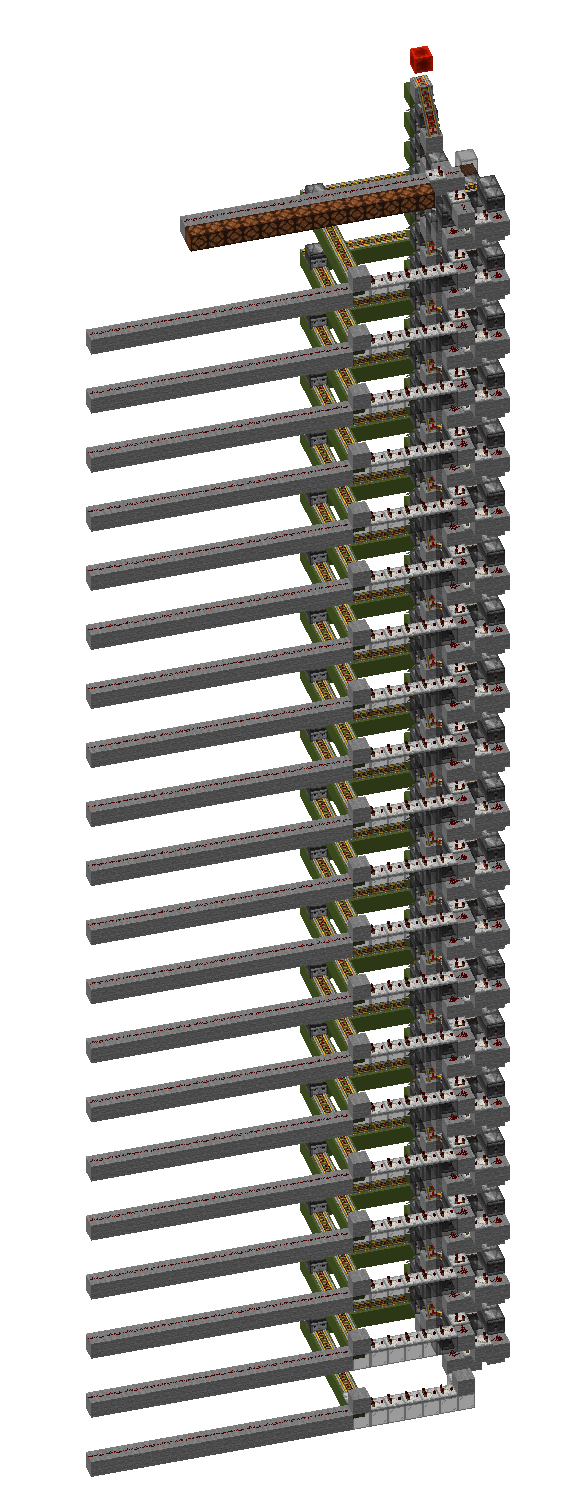
\includegraphics[width=0.30\textwidth]{area_render_3_copy.png}
    \caption{\centering Instant Upwards Comparator Wire}
\end{figure}

% For wide tables, a single column layout is better. It can be switched
% page-by-page.
\onecolumn

\section{Device Specifications}

\begin{table}[h]
    \caption{Device Specifications}
    \begin{tabularx}{\textwidth}{l | c c c | c | X}
        \thickhline
        \textbf{Parameter} & \textbf{Min.} & \textbf{Typ.} & \textbf{Max.} &
        \textbf{Unit} & \textbf{Conditions} \\
        \hline
        Throughput  & 8 & - & - & gt & Normal Usage \\
        \hline
        MC Version & 1.16 & 1.17.1 & - & MCV & Latest version at time of writing: 1.19.3\\
        \hline
        Dimensions & & 10 x 86 x 24 & & Blocks & \\
        \thickhline
\end{tabularx}
\end{table}

\section{Testing Data}
\begin{table}[h]
\caption{Executed Tests}
\begin{tabularx}{\textwidth}{l | X}
    \thickhline
    \textbf{Test} & \textbf{Result} \\
    \hline
    Throughput test & Device was able to function with 8gt clocked input. \\
    \thickhline
\end{tabularx}
\end{table}

\section{Download Information}
\begin{table}[h]
    \caption{Download Information}
    \begin{tabularx}{\textwidth}{l | l | l | X}
        \thickhline
        \textbf{Identifier} & \textbf{MC} & \textbf{File} & \textbf{Description} \\
        \hline
        WI02 & 1.17.1 & WI02\_Instant\_Upwards\_Comparator\_Wire.litematic & Schematic of device. \\
        \hline
        \thickhline
    \end{tabularx}
\end{table}

\end{document}


